\chapter{Space, Place and Infrastructure}
\label{chap:SpacePlaceInfrastructure}

This chapter presents how previous research has explored and examined the qualities of space and place, people's relationships to them and how these factors have influenced educational theory and practice. I also examine how the Human Computer Interaction (HCI) research community has approached this as a design space, particularly through the lens of the Digital Civics agenda \citep{Olivier2015}.

\section{Space and Place}
\label{sec:SpaceAndPlace}

While ‘space’ and ‘place’ are often used interchangeably in everyday discourse, Yi-Fu Tuan and his peers argued that they have quite different meanings: while space might describe the physical properties of a location, place is a metaphysical concept created by human meaning attributed to that space \citep{Tuan1978}. While many of his contemporaries treated geography as an exact and literal science of the physical properties of the earth, Tuan positions it within a more humanistic framing, proposing the treatment of geography as more of a social science. He argues that space is perceived by people on a biological level, with our sensory inputs being combined through recognition of intervals and relational distances to support the perception of the physical world---\textit{`Visual perception, touch, movement, and thought combine to give us our characteristic sense of space.'} Meanwhile, he argues that \textit{place} goes beyond mere location---it also carries a social position. He posits: \textit{`What begins as undifferentiated space becomes place as we get to know it better and endow it with value'}. Thus, place is a social, spatio-temporal value, where space and time go together in shaping a person's interpretations. People who inhabit the same physical space may, due to differing past experiences, associate the space with different meanings and values. Spaces mean different things (are different places) to different people---put simply, it's what makes a house a home. Logically, it follows that the more intimate a relationship an individual has with a space, the less abstract their cognition of it becomes: \textit{`The geographer's understanding of space is abstract, though less so than that of a pure mathematician. The spatial apprehension of the man in the street is abstract, though less so than that of a scientific geographer'} \citep{Tuan1978}.

Like Tuan, Relph was a `humanist geographer' exploring the concept and definition of place. In his book \textit{Place and Placelessness} \citep{Relph1976}, he argues that space is more than simply a container that holds places. Relph posits that in order to be able to encourage the making of new places or the maintenance and restoration of new ones, we must first further understand how we experience both space and place and be able to describe what makes a place special. In an attempt to explore ways of representing how space is experienced, he presents a linear continuum of spatial experience. This structure features direct experience (which he describes as pragmatic, perceptual and existential) on one end and abstract thought (cerebral, ideal, intangible) on the other. Relph argues that we encounter these modes of experience in various intensity throughout everyday life, often subconsciously, and each play a part in how we experience space.

On the more abstract side of this continuum, Relph introduces the concept of \textit{insideness}, which describes the relationship someone has with a place. He posits that if someone feels \textit{inside} a place they feel positively about it (e.g. safe, enclosed, at ease). \textit{Outsideness} describes the opposite (e.g. threatened, exposed, stressed), which would often occur when someone feels a division between themselves and their lived environment (feeling homesick, for example). Relph argues that the more `inside' of a place a person feels, the stronger their identity with it will be. He labels the most extreme of these experiences as \textit{`existential in/outsideness'}, where people feel completely at home with or entirely alienated from their lived environment (a given example is someone returning to their home town after an extended period of time, only to find that the place has changed to the extent that they now feel like a stranger).  

Relph also argues that there are qualities and characteristics of place that can affect how we experience them. He claims that environments which provide `genuine experiences' through direct, unmediated access to their social qualities and constructs (e.g. their local heritage) offer an \textit{`authentic'} sense of place. However, Relph claims that this is increasingly being overshadowed in our modern era by an attitude he refers to as \textit{`placelessness'}: \textit{`the casual eradication of distinctive places and the making of standardised landscapes that results from an insensitivity to the significance of place'}. Relph asserts that by undervaluing places' distinctive characteristics, being overly concerned with efficiency and accepting environments which are interchangeable to the point of anonymity, we run the risk of normalising \textit{`inauthentic'} experiences of place. He argues that this could partly be due to how space is perceived at a larger scale--he posits that the identity of a place becomes less authentic the more people share that identity. He gives the example: \textit{`a city presents a different image to those living in its mansions and those living in its slums'}. The `public' identity of the city would involve a consensus understanding of its image, representing the outlooks of it by all communities. The result is something superficial and contrived, likely representing neither of these communities authentically.  The obvious implication of these arguments on HCI research is that when designing for or conducting research within a location, we must become more aware of the social constructs which underpin it, give it value to its stakeholders and create \textit{place}. To better understand these factors, it's likely that we as researchers will have to grow relationships with a place over time through direct habitation, or at least involve existing stakeholders as participants who have ongoing relationships with it. However, this becomes both more interesting and potentially problematic when accounting for Tuan's arguments of the influence of personal experience--because a person's place attachment is formed based upon individual experience, researchers should be aware that their perceptions of place may not align with others', running the risk of inappropriate design decisions if not handled with care. 

\section{Infrastructures of Place}
\label{sec:InfrastructuresOfPlace}
This necessity for a deeper understanding of their design contexts has led researchers to more commonly apply practices such as ethnography, which Dourish defines as \textit{`an approach to social inquiry characterized by long-term immersive engagement with particular cultures in the effort to understand and explicate how they are experienced by their members'} \citep{Dourish2007b}. He argues that through daily participation in everyday practices, ethnography allows researchers to understand what participants in other communities or cultures \textit{experience}, rather than simply what they \textit{do} \citep{Dourish2006}. However, he cautions that the role of the ethnographic researcher is more than simply a collector of data, looking to find `implications for design': he argues that ethnographic research requires individual interpretation and analytic practice, rather than simply observation. He posits that as a result of this, either explicitly or implicitly, ethnographic stories also tell a story about the ethnographer. As such, observations of communities' interactions with place would vary from person to person, corroborating Tuan's arguments regarding the individual's perceptions of the social values of place.

In her article \textit{`The Ethnography of Infrastructure'}, Star reflects upon the ethnographical study of what is frequently very literal and physical (and, in her own words, `boring') infrastructure: she references the sewers and power supplies of cities; the wires and settings of information systems; and the stairs and ramps of building entrances. However, she argues that meaningful ethnographic study of these systems can open up an \textit{`ecological understanding'} of place, and that that infrastructure is \textit{`both relational and ecological---it means different things to different groups and is part of the balance of action, tools and the built environment, inseparable from them'} \citep{Star1999}. In this regard Tuan's place and Star's infrastructure are similar in many ways. Star argues that the study of the physical infrastructure of sewerage, water and power supplies within cities can help one gain insights into distributional justice and planning power (an obvious example of this would be the water crisis in Flint, Michigan \citep{Clark2018}, the cause and response to which has been labelled as systemic environmental racism \citep{MichiganCivilRightsCommission2017a}); studying the wires and settings of IT systems could yield further a understanding of aesthetics and change; and that a keen observation of the usage (or omission) of stairs, ramps and railings can give an impression of institutional attitudes towards---and considerations of---people living with physical disabilities (for example, the staircase outside Vancouver Law Courts [Figure \ref{fig:stairs}] has been described by an accessibility blogger as \textit{`a serious disaster waiting to happen [and] dangerous for everyone not just those with disabilities'} \cite{Wheeler-Hall2017}). 

\begin{figure*}
  \centering
  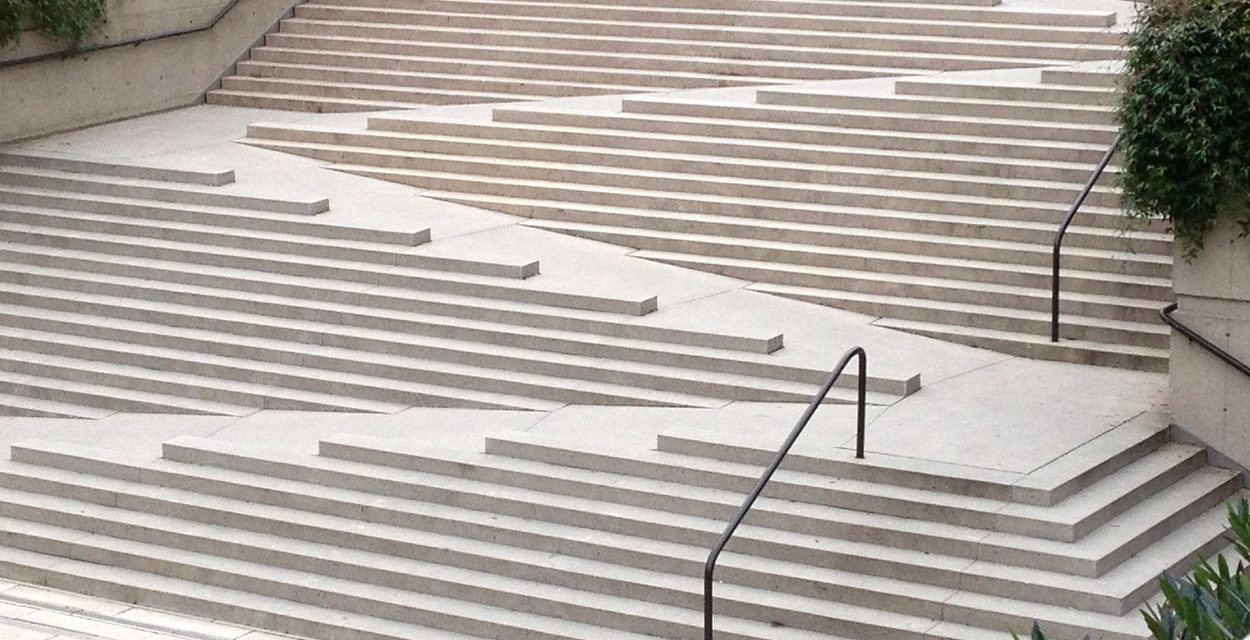
\includegraphics[width=0.8\columnwidth]{images/chapter02/stairs.jpg}
  \caption[Vancouver Law Court staircase]{The staircase outside of Vancouver Law Court, criticised for its lack of accessibility.}
  \label{fig:stairs}
\end{figure*}

Star argues that infrastructure that is boring or even invisible to one person could be another's barrier or topic---for example, while for an able-bodied person those stairs might be fine, an elderly person might immediately notice the lack of handrail along the ramp. She argues \textit{`infrastructure is a fundamentally relational concept, becoming real infrastructure in relation to organized practices'}. Star recalls that few participants in one of her projects utilised the final system that her team designed, despite the researchers following the principles of participatory design throughout the process. They identified that this was not because of usability issues with the interface, but rather how their design was a poor fit with the infrastructures the participants had to work with. The article highlights that the study of infrastructure in an ethnographic enquiry can uncover tacit conventions of everyday practices, allowing the unpacking of relationships between different communities, interest groups and perspectives.

Dourish built upon Star's work, highlighting that as computation increasingly moves away from the context of desktop computing and into the everyday environment, HCI designers must concern themselves with where their technologies are being used and design accordingly \citep{Dourish2006}. Dourish and Bell note that spaces don't just simply comprise of their physical properties, but also of different social, institutional and historical layers of infrastructure \citep{Dourish2007}. They claim that these infrastructures are both embedded into social structures whilst also serving as structuring mechanisms themselves. Infrastructures such as street names, regions, traffic flows and calls to prayer shape a person's experience by making it meaningful in different ways, but are themselves moulded over time into configurations which support social practice. In short, these infrastructures are the fundamental elements through which we encounter \textit{space} and form \textit{place}. Highlighting these infrastructures serves as a method to understand the social and cultural practices that occur within a space. The organisation of space becomes layers of infrastructure, through which we experience the world and produce, understand and enact cultural meaning. 

Dourish and Bell conclude with some implications for design: they argue that because space is organized both culturally as well as physically, a cultural understanding of a place can provide meaningful and coherent framing to relate it to human activities. In the context of HCI, the technologies we design can act as infrastructure within a place, with each having varied social and cultural interpretations and meanings. They also argue that technology designers need to be aware that both space and place feature both physical and social boundaries and transitions, and that these are not always things that technology should try to bridge. They claim these boundaries are frequently used by inhabitants as an asset, and that technologies which introduce `seamlessness' can detract from a place's value. Finally, Dourish and Bell argue that because a) new technology can introduce new layers of infrastructure and b) our encounters with places are formed through their layers of infrastructure, introducing new technologies to a location can inherently cause people to `re-encounter' and re-evaluate it as a space and place. In summary: technology can---as a layer of social infrastructure---act as a destabilizing, transformative force in how we experience place, and can affect stakeholders' experiences with place in different ways.

\section{Place-making}

Encounters with these social, cultural and economic infrastructures are especially important for forming relationships with space---a process frequently called `place-making'. This section will cover some of the ways that researchers have approached place-making, including how it occurs; how existing relationships with place can be surfaced or articulated; and how technologies can be configured to support place-making processes.

\subsection{Building Relationships with Place}
Relph describes a number of ways in which a person's relationship with a new place could form, noting that images and identities of place are not produced from a clean slate, but arise from \textit{`a complex and progressive process that assimilates, accommodates and shares experience and information'} \citep{Relph2018}. Building on his concepts of \textit{in/outsideness}, he introduces the concept of \textit{vicarious} insideness---that which occurs when someone engages with a place through their imagination (e.g. through experiencing a place in works of art or reading about it in a book). He claims it is most pronounced when a place's depiction corresponds with our own experiences of places we are familiar with.  Relph notes another, more deliberate form of placemaking called \textit{empathetic} insideness, which is a very deliberate attempt by an individual to understand a place in depth. This requires a \textit{`willingness to be open to the significances of place, [with] the hope to see it as rich in meaning for those whose place it is'}. These factors can coalesce into authentic and self-conscious placemaking, where \textit{`there is sensitivity to the significance of place in everyday life'}, and can be encountered in instances where communities and individuals have invested hopes and ideals in actively making a place for themselves. However, Relph also warns against the dangers of `museumisation'---the simplification and sanitisation of history to create a more palatable ideal. He argues that by highlighting only the best bits of local history, we run the risk of creating a `Disneyfied', inauthentic image of place.

In their review of environmental psychology-based sense-of-place literature, Kudryavtsev et al. note that many researchers suggest that a `sense of place' is a combination of two complementary concepts: \textit{place attachment} and \textit{place meaning} \citep{Kudryavtsev2012}. \textit{Place attachment} refers to the bond between people and places---the degree to how much an individual or people value or identify with a particular place. They note that researchers sometimes split place attachment into two distinguishable components: `place dependence' (the extent to which a place satisfies an individual's personal requirements) and `place identity' (the extent to which a place becomes a part of an individual's personal identity and--at least partly--defines them as a person). \textit{Place meaning}, however, refers to something closer to the humanist geographers' interpretations of place---the meanings that individuals ascribe to settings that they are familiar with, reflecting their environment, social interactions, culture, politics, economics and history. 

Kudryavtsev et al. note that within the context of environmental education, relatively little research has been done on the combined effects of place attachment and place meaning on `pro-environmental' behaviour \citep{Kudryavtsev2012}. However, they hypothesize that a combination of both factors would be more effective at fostering this behaviour than either taken separately. From examinations of previous works, they suggest that place attachment which hasn't placed an emphasis on ecological elements may not necessarily contribute to pro-environmental behaviour---they suggest that also introducing a pro-environmental place meaning could foster this behaviour more effectively. One might also speculate that this could be applied to many other infrastructural elements of place, outside of the topic of environmentalism. For example, someone might not concern themselves with the socio-economic issues surrounding funding the maintenance of a local park, even if they have built a `place attachment' through a dependence on it for walking their dog. Fostering this element within someone's place identity would likely involve introducing them to relevant infrastructure and forming new place meanings. 

\subsection{Technology as a Mediator for Place-Making}
\label{sec:TechMediator}
Relph argues that one of the primary ways to build a relationship with space is through having experiences with it, and notes that the majority of modern experiences of landscapes are mediated by machines \citep{Relph1976}. Having written his book in 1976, the dominant machine of the time was the automobile. He posits that while at the time there was a narrative that cars had separated people from landscapes and places, this was reductive---the availability of the automobile also extended people's mobility and fundamentally changed how they experienced the world by allowing for new options, comforts and experiences with places that otherwise would likely be inaccessible. Similar arguments can be levied for and against the dominant machine of the 201X's---the smartphone. A common narrative is that digital technologies separate us from `the real world' through distraction, and this may be true in many cases. For example, an over-reliance on technology for navigation (e.g. Google Maps) has led many to repeatedly use the same predetermined routes through their local environment, reducing their exploration and limiting opportunities for building relationships with new places \citep{Lochtefeld2019}. But, similarly to the automobile, the increasing ubiquity of mobile technologies has also dramatically increased users' access to information and experiences that had previously been inaccessible. Modern mobile devices act as a portal to places (both physical and virtual) and their stakeholders all over the world.

Giaccardi et al. note that this new prevalence of digital technologies has opened the door for new ways of interacting with heritage \citep{Giaccardi2008}. They claim that by using `cross-media interaction' (the use of multiple forms of both media and technology) to create new socio-technical infrastructures, novel interactions can be enabled between local communities and their places of heritage within authentic environmental settings. These infrastructures allow for new cultural experiences, articulating and exploring existing people's relationships with place in new ways. It could be argued that these experiences open up new opportunities for visitors to build place attachment through empathetic, vicarious insideness. Giaccardi et al. argue that sustaining this knowledge of social relations is a place-making process, which technology can support by supplying communication and interaction spaces in which communities can engage with the physical and social settings of heritage \citep{Giaccardi2008}. They argue that little HCI design had been done with the aim of reinforcing (or recovering if lost) the relationships between communities and their places of meaning, offering that one possible `solution' could be cross-media interactions. These interactions would allow people to \textit{`express their perceptions, interpretations and expectations about the heritage'}, reinforcing a sense of place through repeated interactions over time. They note that of particular importance is making heritage a `living practice': \textit{`giving people active and supportive roles, [engaging] them in connecting to each others' experiences, considering each other's interpretations, and building insights that may lead to new meanings and relationships'}. Additionally, Giaccardi et al. suggest that the use of technical infrastructure alone is not enough to support heritage practice and place-making---they argue that social infrastructure is necessary for the support and regulation of community participation over time. They also suggest that designs in this space should legitimise personal accounts as far as possible, in order to encourage the collection and conservation of resources---many of which are likely to have unexpected value. This is also linked to another important factor that the authors recognise: the participants' sense of ownership over the content, which strengthens their relationship with the heritage and places of meaning.

Highlighting the distinction between space and place, technology can also support `authentic', personal experiences with place without the need to be at the same geographic location. For example, Google Earth VR allows users to explore most locations in the world from a first-person perspective, using a combination of satellite imagery, street-level photography, and machine learning to generate recognisable 3D environments \citep{Google}. Taken as presented, the software is more reminiscent of \textit{space} rather than \textit{place}---the software does not attempt ascribe any emotional connections or value to particular places, outside of featured landmarks (e.g. the Eiffel Tower). It is simply, in effect, an immersive 3D map. 

\begin{figure*}
  \centering
  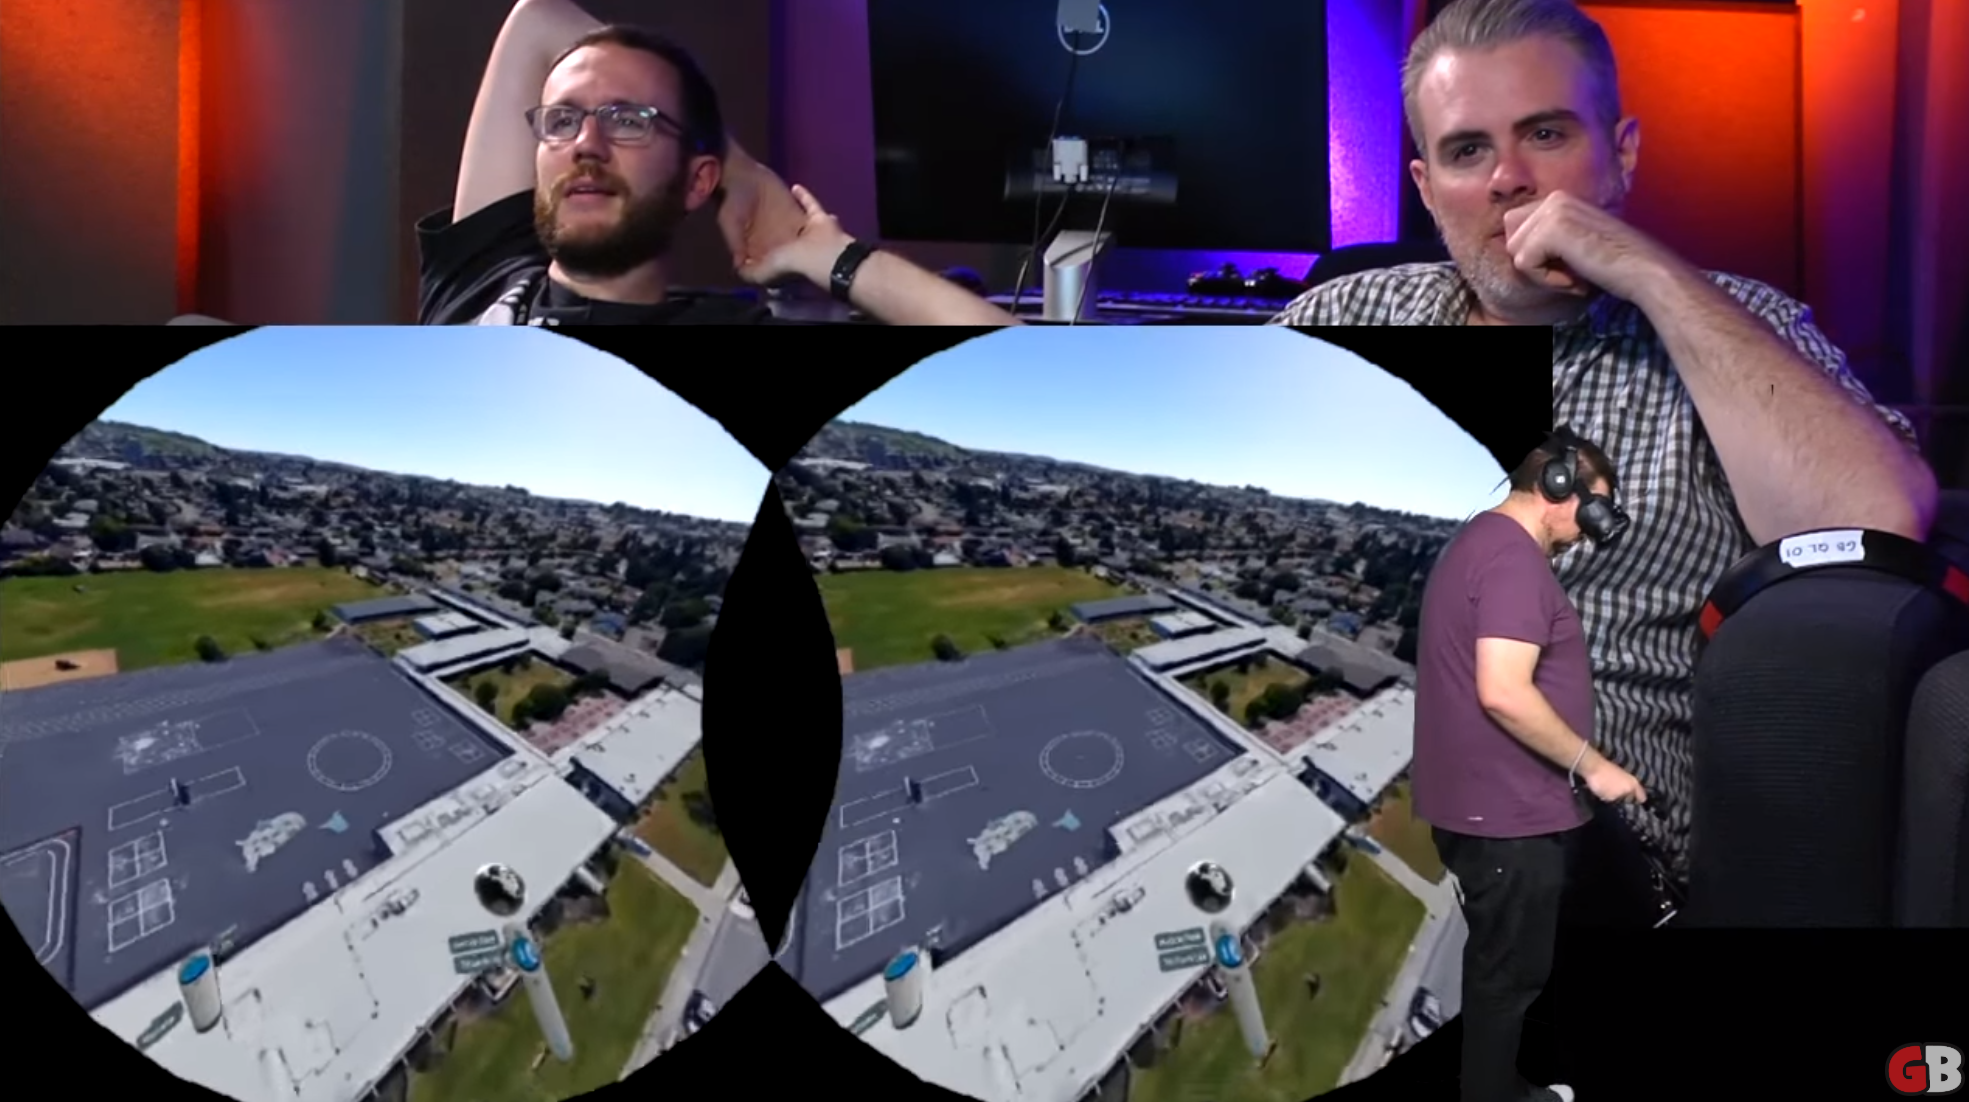
\includegraphics[width=0.8\columnwidth]{images/chapter02/googleEarth.PNG}
  \caption[Jeff Gerstmann showing Google Earth VR]{Jeff Gerstmann shows his colleagues his childhood school in Google Earth VR.}
  \label{fig:googleEarth}
\end{figure*}

However, during a live-streamed internet show, video game critic Jeff Gerstmann demonstrated the software, claiming that the sense of place offered by the experience was \textit{`profound, and almost emotional'} \citep{Gerstmann2016}. Rather than explore far off locations which would be otherwise inaccessible, or the featured landmarks which are of worldwide renown, Gerstmann opted to explore places he already had relationships with: \textit{`Last night I just took my whole commute home, stood in my own backyard.'} During the show, he used the software to visit their company's previous office and even his childhood school, reminiscing about stories from his life [Figure \ref{fig:googleEarth}]. The VR technology allowed Gerstmann to feel like he was present in the authentic environment: \textit{`You know how you do with Google Street View, and you look and say: `Oh those cars are there, it's an old picture' and all that sort of stuff? There's just something about doing it like this that has a really crazy feel, that just looking at Google Earth on a computer just doesn't really do.'} The representation of the world in Google Earth is far from perfect--the generated 3D environment frequently features strange artefacts when viewed up close, and the aerial photography often makes details indistinct. However, this visual abstraction may have even made the software suit better as a reflection tool, as the world was viewed through a strange, dream-like haze reminiscent of faded memories. As Gerstmann notes: \textit{`You get this weird, distorted view of things, which is actually kind of amazing.'} This abstraction wasn't severe enough to prevent him from being able to pin-point specific locations from his past: \textit{`I stood right here in junior high, and played the national anthem on a saxophone'} and \textit{`We found a sealed can of chewing tobacco out here in the [school] field'}. In this instance Gerstmann used Google Earth VR to highlight his place identity, sharing his relationship with place with thousands of others, allowing them to vicariously encounter it through the Internet. Examples such as this highlight the potential for technologies to allow the sharing of different interpretations of space meaning, by giving stakeholders the means to share their past experiences, knowledge and insights to encourage vicarious insideness.

\subsection{Place-Making in HCI Research}
\label{sec:PlaceMakingHCI}

The HCI research community has been investigating this potential for place-making through technology for some time. McCarthy and Wright posit that place-making can be viewed as a dialogical process, in which a person's relationship to a place develops over time through repeated relational interaction and interpretation \citep{McCarthy2005}. They argue that this is a two-way `conversation-like' relationship between the person and their environment, with both contributing qualities which together build a relationship. For example, this might include the person's sensory experiences with the environment, the socio-cultural history attached to it and even the outlook of possible future engagements between the two. The authors suggest that for technologies to help people feel `in place', they should engage at a personal level, rather than treat them as an anonymous entity. 

A good demonstration of many of these concepts in practice can be seen in a study by Crivellaro et al., who worked with multiple heterogeneous stakeholders in the context of a housing estate undergoing urban regeneration \citep{Crivellaro2016}. The area undergoing development had suffered from a poor reputation, fuelled by social deprivation and crime. The researchers worked alongside the site regeneration team, who were aiming to promote a sense of civic pride and community within the estate. Through a series of engagements with current and former residents, they designed walking trails through the area and used a technology probe---in the form of a suitcase containing an audio recorder and written materials (Figure \ref{fig:suitcase})---to collect participants' reflections. Walking trails were chosen as they were \textit{`seen as a means of encouraging a genuine engagement with the environment and stimulated pause and reflection'}. The suitcases and the residents' engagements with them were specifically designed to encourage the participants to convey what they valued about the estate. Participants took turns with the suitcases and exchanged them face-to-face, placing emphasis on listening and sharing recollections and highlighting a diversity of values. The slow pace of this engagement configuration was seen as facilitating \textit{`organic growth'} and the participants developing a sense of ownership of the trail. 

\begin{wrapfigure}{r}{0.5\textwidth}
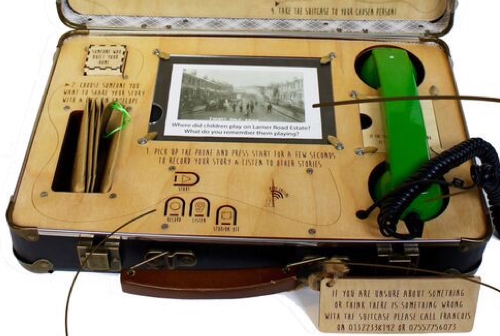
\includegraphics[width=1\linewidth]{chapter02/suitcase}
\caption[Crivellaro et al.'s technology probe]{The technology probe used by Crivellaro et al. to collect participants' reflections about their relationships with place \citep{Crivellaro2016}.}
\label{fig:suitcase} \end{wrapfigure}

The participants were keen to ensure that the trail represented their estate both fairly and accurately---while the area had suffered from negative stigmas which they viewed as being unjust, they were also wary of portraying it in an unrealistically positive manner. This mirrors Relph's concerns around the `Disneyfication' of heritage: glossing over any negative aspects to make the consumption of it more appealing to a modern audience \citep{Relph2018}. Instead, the residents wanted to posit a realistic view which maintained a sense of optimism and used the negative associations they had with their homes more constructively: \textit{`We are doing this because we want people to know that everywhere you go there are going to be problems, and sometimes you can make a negative into a positive thing.'}

Furthermore, the residents viewed their creation of the trail and audio logs as a form of both `anticipatory archaeology' (by documenting the regeneration process) and social curation: \textit{`through immortalising her activities in the towers, she has found a way not to let go, but rather repeatedly etch out a path from past to present, each time her story is replayed and listened to.'} This can be looked at as the participant using the technology probe to safeguard her sense of place from being expunged during the estate's redevelopment, de-coupling her place from the physical space through the use of a socio-technical infrastructure. This wasn't just for her own reflection on her past, either: these memories were recorded so that others could listen to them, allowing her to take a role in other people's place-making with the estate. As the authors note: \textit{`the importance of "giving something back" points to the residents' desire to find value in their stories and actions, and see their contributions as having a wider and lasting impact.'} The participants were re-constructing place identity by using the stories of those who contributed to it.

This can be seen to support McCarthy and Wright's positioning of place-making as a dialogical process \citep{McCarthy2005}: the participant is attempting to continue the conversation. Potentially as a way to make up for `losing' the estate as she knew it, the participant was creating further dialogue with future residents about her experiences of place. Indeed, throughout the study, the authors highlight the heterogeneous nature of the stakeholders and their experiences and opinions. The engagements were designed to highlight these differences while using the estate as a `common ground' with which all of the participants were familiar. The authors argue that collecting a diverse set of accounts that \textit{`enact place over time'} can open a space for more genuine portrayals of community. As McCarthy and Wright argued, the relationships between the estate and the stakeholders were seen to be built up on past experiences, the current situation and the outlook for possible future engagements. The participating stakeholders often had their own motivations and agendas (e.g. showing that life on the estate was generally more positive than its reputation would have suggested), surfaced by the probes thanks to their engagement on a personal level, recognising the participants as individuals.

McCarthy and Wright also note that mobile devices are particularly well suited to engaging people on this personal level: by their nature, phones are an intrinsically personal device, and as the authors argue \textit{`allow people to capture the intimacy of interpersonal relations while moving from one place to another in a public sphere, blurring the traditional boundaries between public and private, intimate and extraneous'} \citep{McCarthy2005}. As an example, the authors cite \textit{RIOT!1831} \citep{Blythe2006}: an interactive play which used mobile technology to connect participants with the past version of their environment. McCarthy and Wright claim that the participants enjoyed having a private experience in a public place, afforded by the nature of the phones' handheld form-factor. They also note the participants' appreciating being in the authentic environment, with them valuing being within the `set' of the play. This concept could also be applied to Gerstmann's experiences with Google Earth VR, which elicited emotional reactions to visiting places from his life experiences in an `authentic' (if virtual) place. Interestingly, Google Earth VR was also similar to \textit{RIOT!1831} in that it allowed for private exploration and reflection in digitised versions of public places (e.g. being able to privately explore public streets which would ordinarily be crowded).

CrowdMemo was another project which used mobile technologies as a part of the place-making process \citep{Balestrini2014}. During the study, school children in Santa Fe, Argentina created video micro-documentaries using smartphones. These documentaries were about places and events important to the local community, and comprised of interviews featuring elderly people sharing their memories with the students. The documentaries were made available online, and accessible by scanning QR codes printed on commemorative plaques installed at places featured in the videos. From a place-making perspective, the researchers noted that the memories collected by the students were \textit{`imbued with features of the local identity, and publicly displaying them led to reflection on locations in the town and why they are relevant to the community's heritage'}. One of the participants claimed that the created documentaries being personal and relatable (and arguably, as a result, more authentic) helped promote reflection: \textit{`it's not about some texts and paragraphs put together by a historian, it's about the testimony of those who gave life to many of the situations in our heritage.'} The place-making impact of the project for local places of extended beyond the members of the immediate community, too: the school's headmaster noted that visitors to the town ask about the QR codes, and the community members use them to promote their culture at all times. 

Balestrini et al. conclude the paper with some recommendations for HCI researchers conducting community technology projects, some of which may be helpful within a `HCI for place-making' context. They recommend following action research principles: involving community stakeholders in the conception and running of the intervention and ensuring that it provides some value to each stakeholder. They argue that these were key factors in promoting a sense of community ownership over the project, with their stakeholders involved from the outset (to the point where the participants actually initiated the collaboration with the researchers). However, the authors note that a sense of ownership of the project would not have been enough to sustain engagement with it---they argue that this was achieved by providing value to all of the involved stakeholders (i.e. valuing the elderly participants' life experiences, giving the young students new technology skills, supporting the teachers in running an innovative educational project). Additionally, they recommend using existing, off-the-shelf technologies in novel ways, rather than introducing new, novel technologies. They note that many of their students already owned smartphones and therefore knew how to operate them, and were excited to be able to use these familiar devices in new contexts with a new set of skills. Reducing the skills barrier and the amount of new technical infrastructure required to participate helped make the project more sustainable. Balestrini et al. also suggest facilitating a range of face-to-face social encounters can lead to discussion and ongoing engagement. A given example is that the encounters between the children and the elderly participants was recognised as one of the most important elements of the project, as it meant that the elderly participants knew that their life stories were being valued. This value of face-to-face encounters is echoed in Crivellaro et al's study, for which the technology probe's integration into the project was designed to encourage face-to-face interactions between participants with different life experiences.

Through the results of their `Community Historians' project, Fox and Le Dantec explored how participatory technology design undertaken with communities could be better configured to support civic engagement and community empowerment \citep{Fox2014}. They found that their their initial approach was more in their interests as researchers than in the interests of their participants, who had been marginalised and particularly disillusioned with academia. In response, the researchers re-framed their workshops to be more clearly and immediately advantageous to the community members that they were working with. This involved both backing away from immediately pursuing their research goals and meeting with community leaders in order to identify ways in which the project could benefit the community members. In response to the community's negative past experiences with academic institutions and their concerns that they were once again being reduced to simple objects of study, the researchers even stopped referring to them as `participants': instead, they were highlighted as collaborators through the use of the term `Community Historians'. With input from the community leadership, the researchers held a series of design workshops exploring how the use and creation of technology could empower residents in the articulation and performance of community identity. The workshops featured `Critical Making', where non-expert workshop participants had the opportunity to take a hand in the creation of device hardware from `raw' components (e.g. camera sensors, motherboards). This was done as a means of promoting reflection about the potential usage of technology within the community, with the authors arguing that a DIY approach can give non-experts a fast-track to unpacking ideas for the potential uses of technology. 

Fox and Le Dantec showed the Community Historians how to make portable cameras which automatically captured images upon detecting movement. However, some were uncomfortable using the cameras, as they were similar in function to the surveillance cameras used by the local authorities (who were seen as not having the community's interests at heart). This clash of researcher expectations with participants' reality is reminiscent of one of Star's projects (\cite{Star1999}, discussed in \ref{sec:InfrastructuresOfPlace}), where the project's solution was a poor match for existing infrastructures in the participants' workplace. The Community Historians project demonstrates that this can also occur with socio-economic infrastructures, not just physical and digital ones. This project was still successful thanks to the goals of the design process: rather than be `product/technology-focused' encounters, the workshops explored what those encounters would have aimed to achieve and how those goals could be accomplished. Rather than focussing on an end product, they worked towards identifying and developing processes to support community practices and empower them in \textit{`in the face of authority and power differentials'}. The authors reflect that HCI design interventions in community contexts need to respect and engage the community on its own terms, acting as a \textit{`balance against trends of rationalization and a rhetoric of disruption that underpin reductive moves to treat all communities the same.'} This argument falls in line with Relph's concerns about `placelessness' (\cite{Relph1976}, discussed in \ref{sec:SpaceAndPlace}), where he argues that by treating places (and---we can intuit---the communities which form around them and give them meaning) interchangeably or at too large of a scale results in `inauthentic' experiences of place. Having a false or incomplete picture of a place's infrastructures can lead to inappropriate design decisions, as seen in Star's unsuccessful project. Fox and Le Dantec present a convincing argument for the fundamental advantages of truly participatory design: involve and emphasize the agency and perspective of community members from the outset, as they are the ones best positioned to inform the design process. As the authors posit: \textit{`a mode of intervention that is based in community practice shifts the power to the community, so that it is not technology and data usurping local influence and ability, but instead technology and data selected in ways to support, preserve and amplify local influence and ability'}. In short, the researchers found that forming partnerships with communities and co-developing alongside them can be an effective way to encourage the articulation of an authentic shared community identity. 

\section{Digital Civics and the Spatial Citizen}
\label{sec:DigitalCivics}
Research held as part of the Digital Civics agenda frequently engages with the socio-economic relationships between communities and place. This section will give a brief synopsis of the Digital Civics agenda; how various Digital Civics projects have engaged with space, place and citizenship; and the concept of the `spatial citizen'.

\subsection{The Digital Civics Research Agenda}

As a result of the economic crisis and resulting austerity measures enacted by the UK government over the last decade, many local authorities have been forced to implement severe cuts to their public services (including--but not limited to--waste management, transport, parks and recreation, education and social care). Olivier and Wright developed the Digital Civics research agenda at Culture Lab (later renamed to \textit{Open Lab}, where this research took place) as a direct response to these developments, claiming that as a research group in a civic university (one which is \textit{`embedded in, and responsive to, its local context'}) they were `compelled' to reflect on how their HCI research could be of use and value to the local authorities and citizens \citep{Olivier2015}. Prior to the Digital Civics agenda, Culture Lab's research had been human-centred and participatory, providing systems and services which were both meaningful and helpful. However, they reflected that their work had been detached from the local context---the research often \textit{`failed to extend beyond the confines'} of their projects, meaning that it frequently could have been done anywhere. They also realised that they were only working within (and, as a result, proliferating) the status quo of service delivery from institution to citizens: they were giving people some input on the design of products, but in a way which still supported the framing of public services as being something `done to' citizens without providing any alternative models. Digital Civics moves away from framing citizens as consumers and towards a model where citizens can take an active role within participatory systems, thanks to new forms of relationships between citizens, businesses and local authorities. Olivier and Wright admit that meaningful, systemic change such as this will take significant amounts of time. Even within the smaller scope of research projects, they posit that the development of long-term relationships between researchers, citizens and local authorities will be necessary if new relational models are to be realised and the potential roles for technology within them discovered.

\subsubsection{On the Dangers of Libertarianism and the Impacts of Big Society}
Before continuing, it is worth mentioning that Olivier and Wright note that there is also a danger of the Digital Civics agenda being warped or misconstrued as \textit{`finding ways of making citizens do it for themselves, or dismantling public service provision'}. Digital Civics was imagined in the context of a period of austerity. As a part of this, many changes were put in place by the UK's conservative government under the guise of localism---part of David Cameron's `Big Society' initiative which purportedly aimed to give local authorities the power to undertake local solutions to local problems, rather than continue to centralise power in Parliament. This agenda was ratified in the Localism Act of 2011, which de-regulated and/or removed many of the constraints related to local issues of housing and taxes \citep{MinistryofHousingCommunities&LocalGovernment2011}, and coincided with a number of austerity measures put onto public services and placing greater emphasis on volunteerism. While the principle of de-centralisation was seen as agreeable across much of the political spectrum, the `Big Society' approach was met with public scepticism. Polls found that over half of respondents thought that the Big Society measures were `just an excuse' to save money by cutting public services, and that only around 10\% thought that Big Society would be a success \citep{Ferragina2017a}. Furthermore, while the restructuring put in place by localism measures relied on more pro-active and engaged citizenship from the public, some argued that not enough resources were allocated to supporting this citizenship actually occurring. As Rogers argued at the time: \textit{`Most of the political problems [the Prime Minister] faces, from cutting crime to reducing obesity, can only be met if residents and citizens play their part. Yet the state has so far invested very little in teaching the skills that could help people make a contribution'} \citep{BenRogers2010a}. This lack of support meant that citizens who wanted to take advantage of the powers given by the Localism Act in areas such as town planning had to invest considerable time and effort, as their output was to be judged to the same level as professionals \citep{BBCSundayPolitics2013}. These expectations of large amounts of free time for research and volunteering would exclude many from the empowerment promised by the legislation, particularly those who had already been most impacted by cuts to social services and were likely to be time-poor.

It is within this context of volunteerism in the stead of well-funded public services that Digital Civics must walk a thin line: between supporting citizens living in the results of austerity and supporting the austerity measures themselves. While in some cases there may be a danger of Digital Civics projects being seen to re-configure the services provided by local authorities to enable a `small government' model, this is is not the intention of the agenda (at least, as I have read it). This libertarian approach (in the contemporary and primarily American sense) is completely contrary to the motivations behind starting the research agenda in the first place: mitigating the damage done by conservative austerity politics upon public services. Instead, Digital Civics projects should aim to strengthen relationships between citizens and local service providers: instead of reducing the role government has within the lives of each citizen and relying on a `DIY' approach, it should aim to empower citizens to have more involvement and agency within their government's processes. This key distinction means that rather than designing in preparation for the permanent loss of public services, Digital Civics technologies should work to mitigate hardships inflicted by austerity measures in a way which also implements improvements for when these measures eventually come to an end. 

\subsection{Digital Civics and Place}

There have already been several projects within the scope of the Digital Civics agenda which are related to the use of technologies within space and, more importantly, place.  

\subsubsection{PosterVote}
While the PosterVote project \citep{Vlachokyriakos2014} predates the publishing of Olivier and Wright's declaration of the Digital Civics agenda \citep{Olivier2015}, it nonetheless fits within it thematically. The project explores how low-cost technologies could be utilised by communities to support grassroots democracy and social action. The PosterVote system consists of two components: a low cost, lightweight piece of hardware, consisting mostly of buttons and LEDs; and a simple piece of printed paper, onto the back of which the hardware is stuck. A question and up to five responses is printed onto the paper, with each response having one of the hardware's buttons underneath. The system simply records users' choices, which can be reported back through a machine-readable series of LED flashes and beeps. 

The motivation behind the project stemmed from how most uses of technology for civic engagement (e.g. responses through Twitter, showing discussions on public displays) frequently require technical knowledge and are `mostly initiated or managed by local political organizations and local councils'. As a result, these institutions are still the ones driving agendas, and usually only using these technologies as consultation tools to increase perceptions of efficacy. Vlachokyriakos argues that the high cost and top-down nature of these systems make them `inappropriate for activism'. In response, PosterVote was designed to support the diverse viewpoints of activists and stakeholders by removing the need for technical skill and significant funding. Furthermore, the nature of the design harnesses different engagement levels of people within communities: individuals who are the most engaged and are willing to put more effort into a project may choose to set up their own PosterVote instance, while less engaged members can simply use the devices to share their views or make use of the data others have collected.

One of the main reported advantages to PosterVote is that is can operate within relevant space and place---the nature of the technology means that it can be placed in a location relevant to the question being asked, and that people's participation with the system can be configured according to where and how it is deployed. Participants noted: `\textit{The thing about having it on a lamppost is it's directly relevant to that particular position. [We didn't deploy it in the supermarket as] the sample population was too broad, we wanted it to be people who used Coniston Street}'. Furthermore, the authors argue that the low cost of the posters initiated discussions about their ownership: some participant groups treated the deployments as an effort to be owned by the community (without making any real distinction between the posters' organizers and the wider community), while others were cautious about democratising the process too far and kept a more rigid hierarchy. 

\subsubsection{FeedFinder}

FeedFinder \citep{Balaam2015} is a smartphone application designed to support breastfeeding women in finding, reviewing and sharing public breastfeeding-friendly places. The application allows users to add locations to a map, and review and rate them on five categories: comfiness, cleanliness, privacy, baby facilities and average spend. Reviews are public, meaning that other women can see how places have been rated to make more informed decisions about where they choose to breastfeed.

FeedFinder was designed as a response to a perceived lack of practical and moral support for breastfeeding in public spaces, which results in many women choosing to only breastfeed in private locations (frequently meaning they're more or less housebound). The choice of rating categories is reflective of what the participants in the researchers' design workshops thought to be `\textit{what qualities of a place were important to a positive public breastfeeding experience}'. Some women even used the system to try and effect change: for example, one participant showed the application to a department store's manager, comparing them to a competitor's ratings as a way to get them to improve their facilities. 

Also discussed was the tensions between user expectations of available content and being entirely reliant on grassroots, community-generated data. One participant noted: `\textit{I love the idea, but there's no places listed! [...] You shouldn't just rely on user submissions as people won't use an app with no content.}' This highlights the need to `get the ball rolling': as Vlachokyriakos noted \citep{Vlachokyriakos2014}, systems should support the different levels of engagement in participants. Having no pre-loaded data available means that more passive users won't engage with the system--at least until it has been populated by others. However, providing an initial `authoritative' dataset is at odds with the app's intention to promote community generated data.

Despite this, FeedFinder served as a tool that facilitates the collection and sharing of `\textit{lived experiences}' of breastfeeding in public, and the comparison of these experiences on a local, regional and national level. This supported participants in not only finding more comfortable places to breastfeed, but also provided a way to compare lived experiences to the presumed rationality: that the public is not supportive of breastfeeding in public. These surfaced lived experiences acted as evidence for publics who wanted to affect civic action and real social change.

\subsubsection{AppMovement}

AppMovement is a platform which enables the promotion, design, production and deployment of community-commissioned mobile applications. Using a website, users are able to propose a idea for a location-based review mobile app (e.g. "Safe places to fly your drone"). In order to show that the app has a potential audience, the user then needs to promote their application and try and get others to note their support. If the app gets enough of a following, it is promoted to a collaborative design stage, where people who pledged their support to the app contribute or make suggestions towards its production (e.g. providing text, iconography, place qualities which should be rated). Once finished, the app is automatically built and published to the app stores.

AppMovement builds upon the concept of FeedFinder (a platform supporting a community around a specific issue in reviewing places according to certain criteria) by allowing communities to commission similar applications, bespoke to their own contexts and requirements. It extends the `grassroots', community-contributed nature of FeedFinder into the application itself---as well as the place review data within each app being community generated, the application itself was similarly proposed, produced and promoted by a community of interest. The authors note that communities had already demonstrated that they're capable of (re)appropriating technologies for their own purposes, however issues of cost and technical know-how frequently prevent them creating their own bespoke solutions. AppMovement democratises the creation of mobile software and serves as a blend between PosterVote and FeedFinder, lowering the cost and technical requirements of producing technologies which can be used by communities for their own requirements, independent of top-down institutions. The authors note that this process led to a sense of ownership and stronger engagement: `\textit{Proposing an idea leads to a sense of ownership of it. The result of this sense of ownership is the increased motivation to promote the concept and engage the community in the appraisal of the idea.}'. Furthermore, they argue that the democratising of the app creation process opens it up for appropriating by communities, allowing them to `\textit{more accurately address [the] issues they face}'.

The process of commissioning support for a proposed application also helps address the issue of a lack of seeded content, as seen in FeedFinder. Requiring the initial proposing user to gather support for their application not only guarantees that the application will have an initial audience, but it also pulls in the community members who are most likely to strongly engage and create content. Involving these individuals in the platform before it launches (rather than having them find it organically post-launch) makes it more likely that more content will be created in the early stages of the app's life.

\subsubsection{WheelieMap}

WheelieMap \citep{Kirkham2017} is another Digital Civics project which explores how digital space-based technologies can support civic advocacy. The WheelieMap platform is designed to support wheelchair users in identifying, documenting and reporting areas which have accessibility issues. The mobile app does this through recording and uploading a combination of motion data, video clips and GPS location data. When combined with qualitative user reports, the system can empower wheelchair users to map inaccessibility and advocate for improvements. This approach improves on existing solutions, which frequently rely on expert documentation (which is expensive), purely automatic systems (which lack qualitative assessments) or `offline' community efforts (which frequently lack actionable evidence for decision makers). 

When reflecting on their experiences with the system, some participants noted that it offered a potential for sharing their point of view and assisting in empathy with the wider public: `\textit{I think it would be really good to show the general public things they otherwise wouldn't think of [...] if you don't experience it yourself, you just don't think about it sometimes. This terrain would be really easy to walk along; you don't realise what it would be like for someone in a wheelchair or with a pram.}' In this context, the technology was used as a tool to assist in communicating to others the participant's interpretation of place (particularly the infrastructures within it, such as paths), and how it could be improved. The authors note that future efforts will need to account for the disparate viewpoints and goals of those who collect and utilize the data, as well as retain a community which is willing and able to engage with the system over time.

\subsubsection{Data:In Place}
With the amount of data being generated regarding places and people increasing daily thanks to developments such as smart cities, questions have risen regarding how such data could be made openly accessible for use by citizens. Data:In Place is a web platform designed to support the open access and sense-making of data for the purpose of civic advocacy by citizens, enabling effective action in relation to place-based issues and concerns backed by relevant data \citep{Puussaar2018}. The authors worked with a group of residents interested in starting a Neighbourhood Plan, a process introduced through the Localism Act as discussed earlier. The Data:In Place platform supported these citizens in using data as evidence for their civic action. Previously there had been technical and knowledge barriers in place which had distanced them from using it effectively, relying on third-party professionals and raising issues around dependency, economic exclusion and misrepresentation. The authors argue that being able to easily access data through the platform also supported participants in exploring local issues and more deeply understanding their communities.

\subsubsection{ThoughtCloud}

ThoughtCloud \citep{Dow2016} is a feedback system, designed to be deployed in situ where voluntary and community care organisations deliver their services. The system supports both quantitative and qualitative feedback, through the use of Likert scales and the recording of video and audio messages. Suggestions for feedback topics can be configured by the event organisers by them supplying a set of questions. ThoughtCloud was motivated in part by the fact that stakeholders who use and rely on certain services are frequently under or misrepresented in existing feedback pipelines, with reasons ranging from stigmatisms of particular services, tokenism, or even participants fearing imperilling their access to those services. The authors argue that the fact that certain groups are excluded refutes the political ethos that `everyone has a voice'.

One of the study's findings was that while some of the more structured responses were of limited use (due to the participant being overtly guided by a third party or a leading question), some of the more unstructured qualitative data was seen to provide `\textit{richer accounts of personal experience of the provided services, and how people saw themselves as members of a community.}' This suggests that participant-led free-form audio and video recording could be a good medium for gaining insights into stakeholders' relationships with the social infrastructures they engage with, and how they position themselves within a community.

\subsubsection{Community Conversational}

Community Conversational \citep{Johnson2017} is a Digital Civics project with direct ties to the issues surrounding the UK government's localism measures discussed earlier. The project focuses on community organisations' and local authorities' consultation engagements with local residents. These organisations had a responsibility to involve local residents in consultations and provide evidence for both the fact that these engagements took place, and that the views and opinions raised by residents were being taken into account in the decision making process. In keeping with the increasing reliance of volunteerism due to cuts to local authorities' funding, running these engagements had become the responsibility of volunteer-based organisations. The researchers identified that these consultations frequently failed to capture rich insights from participants, due to the volunteer groups lacking the resources and research experience necessary to effectively capture and analyse data produced during the sessions. Other issues included poor contextual data collection and participants cross-talking and dominating discussion. 

In response, the researchers produced Community Conversational---a workshop activity which took the form of a board game, augmented with video recording and an online data repository. The game structured conversations using cards to control turn-taking, which addressed issues around conversations being dominated by individual participants. Game pieces could be placed on a map, with the system tracking their placements. The recorded audio and video were automatically cut into chunks around participants' interactions with the pieces, making them easily searchable during analysis but still retaining a good amount of the conversation context.

The researchers report that when interacting through the game, the participants seemed more willing to listen to and even empathise with alternative viewpoints. This could likely be attributed to the conversations being structured by the game's rules, ensuring not only that all participants got a chance to speak, but also that the other participants had to listen.

While the participants valued the more open nature of the conversation---thanks to it not `\textit{being bound by and driven by council officers}'---the decision making facilitators struggled to make use of the more more open qualitative data. The researchers noted that despite the collected data being `rich', the decision makers saw it as being of limited use, having previously aimed to collect quantitative results as evidence of support for previously identified solutions to a given issue. The authors argue that this points towards the organisations recording the opinions of local experts as a tokenistic series of bureaucratic tick boxes, rather than including them in meaningful consultations. This was further evidenced by the council representatives using the data purely in relation to predefined issues, limiting the practical value of a rich data set. 

Comparing the findings of Community Conversational with those of WheelieMap and ThoughtCloud makes it clear that even if consultation participants are contributing rich insights about their use of space, the perceived value of participants' sharings on place is limited by the way they are analysed and responded to.

\subsubsection{Gabber \& TalkFutures}
The Gabber project explicitly aims to tackle this issue by supporting stakeholders in contributing directly towards the collection and analysis of qualitative data \citep{Rainey2019}. The Gabber mobile app supports users in collecting spoken audio data, with participants responding to pre-defined prompts written by the research co-ordinators. Participants can either record themselves or others responding to these topic prompts, supporting qualitative data collection which is distributed, large-scale, low-cost and participatory. With the interview participants' explicit consent, audio recordings are then made available on the Gabber website for others who have been involved with the project to listen to, highlight, tag with themes and comment upon. In this way, stakeholders partaking in public engagements are able to contribute throughout the entire process, and are given more transparency around how their data is being used.

A fork of Gabber, TalkFutures, was developed as a component of Strategy 2030, a research project within the International Federation of the Red Cross and Red Crescent (IFRC) which aimed to understand the issues and challenges which the Federation would face in the near future. Through workshop engagements with teams and individuals throughout the IFRC (from volunteers in Mexico to leaders in Geneva), several key themes and issues were identified which members believed the Federation should prepare for. These included topics such as the impacts of rising sea levels due to climate change, and mass migration with the increasing trend of urbanization. Once these issues had been identified, the next step of Strategy 2030 was to collect ideas of how the IFRC needed to change in order to best prepare for them. The TalkFutures app was created and deployed to collect these ideas from IFRC members across the globe.

As with Gabber, TalkFutures made it easy for participants to contribute semi-structured, qualitative audio data (e.g. in the form of interviews). The application also allowed participants to control others’ access to their contributed audio recordings, with participants within a conversation being able to withdraw their consent, even after it has been uploaded. Uploaded audio recordings were made available on the TalkFutures website, where they could be filtered by discussion topic or even which National Society the participants worked in. By the conclusion of the Strategy 2030 investigation, members from 86 different National Societies contributed recordings using the application.

The approach taken by Rainey et al. in both Gabber and TalkFutures is reminiscent of Fox and Le Dantec's `Community Historians' project (discussed in \ref{sec:PlaceMakingHCI}), in that stakeholders contributing to the research are treated as collaborators rather than participants. While Community Conversational encountered institutions simply engaging stakeholders as a sort of tokenistic gesture to justify previously made decisions, the collaborative structure of Gabber almost precludes that---stakeholders are able to see each others' data, contribute to its analysis and hopefully more easily understand how the researchers reach their final conclusions. These projects highlight that including stakeholders to give creative input throughout an engagement process is key to gaining the richest understanding of issues within place.

\subsubsection{Remix Portal}

Remix Portal is a web platform designed to connect schools with musicians within the local community through the teaching of music remixing \citep{Dodds2017}. The tool is used within school music lessons, allowing children to place effects and mix the individual instrument stems of given tracks created by local musicians. After remixing, children are given `show and tell' feedback through the web portal: feedback can be left through the website directly onto the remix, and the mix board's controls manipulated to demonstrate suggested changes to the learner. This feedback can be left by fellow students, teachers, or---most significantly---the original musicians. As a result, Remix Portal provided a platform upon which schools were able to directly connect with local experts within nearby communities. This gave the students a greater appreciation of their local music scene, as well as a realisation that it was possible to create great creations without needing to have the opportunities given to the biggest stars. As one student noted: `\textit{Everyone expects it to be the big famous people that you listen to, but we've got people living nextdoor to us that are just as good.}' The students were also particularly motivated knowing that the original musicians would listen to their remixes, as they wanted to `impress them'. The experts also claimed to benefit from the study from exposure to new audiences, inspiration from the students' submissions and even the opportunity to `pay back' teachers who had previously nurtured their talent.

Remix Portal demonstrated that it's possible for learning technologies to introduce new layers of infrastructure for local knowledge sharing. By taking part and being exposed to local talent and expertise, the students were able to reflect and re-evaluate their interpretation of place within the context of music production, potentially opening new avenues for the students to further explore.

\subsection{Spatial Citizenship}

Outside of the Digital Civics agenda, Gryl and Jekel argue for a greater utilisation of geo-information systems (GIS) in secondary schools \citep{Gryl2012}. However, they first describe two arguments for it that they find unconvincing: first, that secondary education should prepare students for entering the workforce by introducing them to technical tools, and GISs are becoming increasingly prevalent within industry; and second, that spatial thinking is a key competence for problem solving across multiple subjects, supporting students' understanding of the concept of space, tools of its representation and familiarity with related processes of reasoning. Countering the technical argument, they posit that short-lived software skills cannot reasonably be part of secondary education, and that technology tends to simplify as it advances, further reducing the importance of training in specialty software. They are also critical of `spatial thinking', noting that is usually only comprised of geographic elements, denoting a very narrow and limited concept of space. They argue that social elements such as human intent, power and political processes are absent in such arguments for the inclusion of GIS.

{ \RaggedRight
\begin{tabularx}{\linewidth}{ p{30mm} | X X X}
    {\small\textit{Dimension of citizenship}}
    & {\small\textit{Dutiful citizen}} 
    & {\small\textit{Web 2.0 citizen}}
    & {\small\textit{Spatial citizen}}\\
    \midrule
    \small Knowledge 
    & \footnotesize National history emphasizing common experiences and myths; government functions. 
    & \footnotesize Generational histories emphasizing life experiences; finding and assessing credible sources of information outside the official domain. 
    & \footnotesize Spatial embeddedness of social life; constructions of space and deconstruction methods of spatial information.  \\
    \hline
    \small Organisation 
    & \footnotesize Knowing about lobbying, parties, civic groups; reasons to join these. 
    & \footnotesize Role of social networking, reasons to and effects of joining social networks.
    & \footnotesize Geo-communities; effects of everyday application of GI; spatial privacy issues.  \\
    \hline
    \small Communication 
    & \footnotesize Understanding conventional media. 
    & \footnotesize Participatory media skills (e.g. blogging); learning how to reach audiences with digital media. 
    & \footnotesize Participatory geo-media skills: competitive lay mapping, volunteered geographies, learning about the power of maps.  \\
    \hline
    \small Participation 
    & \footnotesize Voting, campaigning and courts of justice. 
    & \footnotesize Identification of paths to join or organize effective peer advocacy networks.
    & \footnotesize Identification of paths for spatial analysis and representation in decision-making processes.  \\
    \hline
    \small Attitudes 
    & \footnotesize Trust in government and institutions of the state. 
    & \footnotesize Empowerment, trust in networks, confidence in participatory skills. 
    & \footnotesize Habit of reflection on own and others' spatial constructions, confidence in participatory skills regarding spatial planning.  \\
    
\end{tabularx}
}
\captionof{table}{Gryl \& Jekel's spatial citizen, compared to the education of other models of citizenship such as the `Web 2.0 actualised citizen' \citep{Gryl2012}}~\label{tab:SpatialCitizen}

Instead, they argue that `spatial citizenship' is their preferred approach for including GIS in secondary education. Rather than configuring the use of technology to prepare students for entering the workforce or meeting scientific requirements, spatial citizenship is centred around the everyday lives of individuals. They claim that education for spatial citizenship `\textit{aims at enabling secondary students to devise alternative spatial scenarios, and to participate competitively in society with the help of GIS}.' Gryl and Jekel argue that such an education is necessary to prepare students to be active `spatial citizens': those who are able to use geographic information systems to \textit{`critically appropriate space by democratic means in order to participate in society.’} In short, it's teaching students how to use spatial data to be citizens, rather than simply workers. The goals of spatial citizenship education---and a comparison to previously existing models of citizenry---can be seen in Table \ref{tab:SpatialCitizen}. In order to fully participate in society, the authors argue that learners should be able to access, read, interpret and critically reflect on information surrounding a space, as well as express and share their own location-specific opinions. Gryl and Jekel argue that citizens' access to and understanding of data can be a society-changing factor: they posit that data can be used to exercise control over others or work towards solving the world's problems, and that the absence of it can allow for such problems to be neglected or hidden---particularly with the construction of `alternative facts' \citep{gryl2018}. The links to the previously discussed Digital Civics projects are obvious---under this context, there is a clear scope for the concept of the spatial citizen to play a role in local knowledge sharing and exposure to existing communities (e.g. Remix Portal), collecting opinions within given areas (e.g. PosterVote), platforming stakeholders' opinions on given topics (e.g. Gabber, Community Conversational, ThoughtCloud), providing data as evidence for advocacy (e.g. Data:In Place, WheelieMap) or the creation of new GIS technologies to meet a community's specific needs (e.g. FeedFinder, AppMovement). An important aspect of civic education is giving the learner the skills and knowledge necessary for active involvement in society, through information sourcing, critical analysis and debate. Highlighting the importance of active citizenship, Walzer claims that \textit{`the passive enjoyment of citizenship requires, at least intermittently, the activist politics of citizens’} \citep{Walzer1983}. Spatial citizenship allows for the re-contextualisation of the above projects into the field of education, exploring how the development of active spatial citizens can be supported through the use of place-based technologies. 

\section{Summary}

This chapter briefly introduced the concepts of space, place and infrastructure, as well as some of the HCI research that has been undertaken to understand how technologies might influence the place-making process.

Place and space are different---albeit related---concepts: while space might describe a geographical area which our bodies can perceive, place is much more abstract, describing the meanings that individuals ascribe to physical or abstract (e.g. online) spaces. Space and place also feature layers of physical and social infrastructure, which can be interpreted on a similarly personal level and can shape how individuals experience place. For these reasons, place-based technologies need to at least be aware of the personal nature of a place, as people's experiences, relationships and interactions with it can be jarringly different.

Our relationships with places are built through experiences with them over time (`place-making'), however the nature of these experiences can change how the relationship develops. For example, a person might subconsciously experience place remotely through seeing it in movies (`vicarious insideness'), or deliberately attempt to understand a place in-depth through more thorough investigation (`empathetic insideness'). Furthermore, these representations of place may be deliberately or inadvertently sanitised through `museumisation', leading to an inauthentic, `Disneyfied' experience of place. Place-making is frequently defined as being made up of two complementary concepts: place attachment (the degree to how much someone values or identifies with a place, from it fulfilling their needs or defining them as an individual) and place meaning (the meanings that individuals ascribe to settings that they are familiar with, reflecting their environment, social interactions, culture, politics, economics and history). 

As place-making occurs through \textit{experiencing} place over time, technology is able to influence the process. While frequently derided as elements that distract from experiencing the real world, digital technologies such as smartphones also provide new place-making opportunities by opening up access to new media formats, discourse and information and places near and far. Technologies have already allowed people to share their personal experiences with and knowledge of place with others, supporting new avenues for building vicarious and empathetic insideness through the sharing of place meaning. Many Human-Computer Interaction researchers have investigated the potential roles for technology within place-making and users' interactions with place and infrastructure. Researchers have repeatedly emphasised the importance of working closely with stakeholders, through co-design and action research methods. Working closely with the individual and the local can grant insight into personal stories and individual interpretations of place and infrastructure, minimising inauthentic representation and inappropriate design. Researchers have also noted the importance of providing value to the stakeholders they work with, and that giving stakeholders a degree of ownership over the project notably increased meaningful engagement.

Finally, I discussed how existing Digital Civics projects have supported and empowered place stakeholders with new methods for knowledge sharing, self-representation and the expression of their needs and values---all of which could be utilised in the place-making process. Gryl and Jekel's `spatial citizen' was also briefly covered, providing an opportunity to re-frame technologies designed to promote place-based citizenry to the field of education.